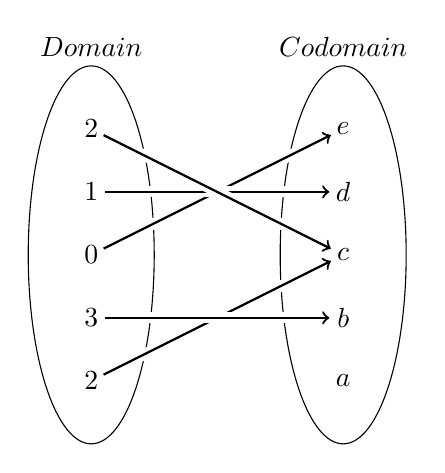
\begin{tikzpicture}[node distance=0.5,scale=0.8]%,alt={arrow diagram of a function}]
% Sets
    % Domain
    \draw (0,0) ellipse (1cm and 3cm);
    % Codomain
    \draw (4,0) ellipse (1cm and 3cm);
% Function
    \foreach \x/\c in {-2/a,-1/b,0/c,1/d,2/e}{
        \pgfmathparse{int(Mod(\x,4))}\let\y=\pgfmathresult;
        \draw[->,line width=4pt,shorten <=5pt,shorten >=5pt,white] (0,\x) -- (4,2-\y);
        \draw[->,thick,shorten <=5pt,shorten >=5pt] (0,\x) node {\y} -- (4,2-\y);
        \node at (4,\x) {\(\c\)};
    }
% Labels
    \node[anchor=south] at (0,3) {\(Domain\)};
    \node[anchor=south] at (4,3) {\(Codomain\)};
\end{tikzpicture}